%
% Maturarbeit von Denis Augsburger und Nicolas Mauchle
%
% Betreuer S. Kuster G. Colins
%
% GIBM 2011
%
% Version 0.3
%
\documentclass[12pt,a4paper,german]{article}
%
\usepackage[left=3cm,right=2cm,bottom=3cm,includeheadfoot]{geometry}
\usepackage[pdftex]{graphicx}
\usepackage{babel}
\usepackage[utf8]{inputenc}
\usepackage{fancyhdr}
\usepackage{lastpage}
%Mathe Paket Denis%
\usepackage{amsmath}
\usepackage{amssymb}

% suppress boxes around links:
%\usepackage[pdfborder='0 0 0']{hyperref}

\usepackage{hyperref}
\hypersetup{
    pdfborder = {0 0 0}
}

%Damit man label setzten kann wo man will
\usepackage[all]{hypcap}
%

\usepackage[stable]{footmisc}
% KOPF UND FUSS ZEILEN
\pagestyle{fancy}
%
\fancyhf[R]{}
\fancyhf[L]{\leftmark}
%
% suppress page number in bottom center:
\cfoot{}
%
\fancyfoot[L]{}
\fancyfoot[R]{Seite \thepage \  von  \pageref{LastPage}}
%
%Linie unten
\renewcommand{\footrulewidth}{0.5pt}
%
\begin{document}
%
%-----------------------------------------------------------
% Title Page
%-----------------------------------------------------------
\begin{titlepage}
\sffamily
\centering
%LOGO 
%
\includegraphics{images/gibm_logo.png}
\includegraphics{images/titelblatt_alternative.png}
%Titel
\vfill
{\bfseries\Huge RSA-Verschlüsselung}\\
\vfill
%Fragestellung
{\bfseries\Large Wieso ist RSA heute noch sicher?}\\
\vfill
Verfasser:\\[1ex]
Denis Augsburger\\
Nicolas Mauchle\\
\vfill
Betreuer:\\[1ex]
{\large Stefan Kuster}\\
{\large Gary Collins}\\
\vfill
\raggedright
\small
Muttenz, 19. Dezember 2011\\[2cm]
\begin{tabbing}
Klasse:\quad\quad\quad \=BMI 4B\\
Fächer: \> Englisch, Physik \\
Schule: \> GIBM - Muttenz
\end{tabbing}
\end{titlepage}

%
%-----------------------------------------------------------
% PLACE TEXT HERE
%-----------------------------------------------------------
\tableofcontents
%
%-----------------------------------------------------------
% EINLEITUNG
%-----------------------------------------------------------
\newpage
\section{Einleitung}
\subsection{Vorwort}
Bei der Themenwahl suchten wir ein Gebiet, welches uns interessiert und in unserem zukünftigen Berufsalltag begegnen wird. Wir entschieden uns für die Verschlüsselung, weil dies in der IT ein sehr wichtiges sowie aktuelles Thema ist. Da die Verschlüsselung zu allgemein definiert ist, haben wir das Thema weiter eingegrenzt und sind auf die RSA-Verschlüsselung gestossen. Diese asymmetrische Verschlüsselung wurde schon früh entwickelt, behielt bis heute ihre Bedeutung und wird in verschiedenen Anwendungen eingesetzt. Mit dieser Themenwahl konnten wir nach mehreren Anläufen auch unsere Betreuer davon überzeugen, dass wir dieses komplexe Thema bewältigen können. 
%
\subsection{Leitfrage}
Der RSA-Algorithmus ist im Jahr 1977 veröffentlicht worden. In der IT hat sich seit dieser Zeit viel verändert. Die Rechner sind wesentlich schneller geworden, es entstanden neue, verbesserte Algorithmen, und durch die grosse Verbreitung des Internets wurden asymmetrische Verschlüsselungen immer wichtiger. In unserer Arbeit möchten wir herausfinden, ob das erste veröffentlichte asymmetrische Verschlüsselungsverfahren auch heute noch sicher ist. Zusätzlich möchten wir verstehen, wie und warum der Algorithmus funktioniert. Um beides abzudecken, haben wir unsere Leitfrage wie folgt definiert:\\
\begin{center}\textit{Wieso ist RSA heute noch sicher?}\end{center}

%
%-----------------------------------------------------------
% Allgemeines über die Verschlüsselung und ihre Geschichte
%-----------------------------------------------------------
\newpage
\part{Verschlüsselung Allgemein}
\section{Sinn und Zweck der Verschlüsselung}
Die Verschlüsselung bzw. die Geheimhaltung von Informationen gibt es schon lange. Die Frage ist, wie kann ich eine Information vor aussenstehende so darstellen dass es für sie keinen Sinn ergibt. Ich, oder andere, mit einem geheimen Schlüssel die Information lesen können. Im realen Leben können wir zum Beispiel unser Haus vor Dieben sichern, indem wir eine Türe mit einem stabilen Schloss einbauen. Möchte man noch weiter gehen, kann man eine Alarmanlage einabauen.\\[2ex]
%
In der Digitalen Welt geht das nicht so einfach. Obwohl man seinen Rechner mit einem Benutzername und Passwort für unbefugte Personen schützen kann, gibt es Techniken, mit der lassen sich ganze Festplatten Bit für Bit kopieren. Hier setzt die Verschlüsselung an. Denn wenn man etwas verschlüsselt auf die Festplatte speichert, kann der unbefugte die gestohlenen Daten nicht brauchen.
\section{Geschichte der Verschlüsselung}
\subsection{Klassische Kryptografie}
Die Kryptographie bezeichnet die Entwicklung von Methoden zur Verheimlichung von Nachrichten.
Solche Methoden wurden schon 3000 Jahre vor Christus bei den Ägyptern verwendet(Hyrogliphen). \\
Die Hebräer haben 600 vor Christus das Atbash entwickelt. Dabei wurde das Alphabet umgekehrt und entsprechend verschlüsselt.
Als kleines Beispiel

\begin{table}[ht]
\caption{Atbash Verschlüsselung}
\begin{center}
\begin{tabular}{|l|l|l|l|l|l|l|}
  a & b & c & d & e & f\\
  z & y & x & w & v & u\\
\end{tabular}
\end{center}
\end{table}


Die Caesar-Verschlüsselung wurde nach Julius Caesar benannt und zur militärischen Korrespondenz im Römischen Reich gebraucht.\\
Dafür wurde damals das Alphabet um 3 Stellen nach hinten verschoben. Aus einem D wird somit ein A. Dieses Verfahren wurde im 15.-Jahrhundert mit einer
Chiffrierscheibe verbessert und ist bis heute noch als Caesar Verschlüsselung bekannt. Die Verschiebung um 13 Stellen wird auch als Rot13 bezeichnet, 
da das Alphabet aus 26 Zeichen besteht, ist die Verschlüsselung und Entschlüsselung bei Rot13 die selbe.

\begin{table}[ht]
\caption{Caesar Verschlüsselung um 3 Zeichen}
\begin{center}
\begin{tabular}{|l|l|l|l|l|l|l|}
  a & b & c & d & e & f\\
  x & y & z & a & b & c\\
\end{tabular}
\end{center}
\end{table}

All diese Verfahren können ziemlich eifach geknackt werden. Da bestimmte Buchstaben in einer Sprache öfter vorkommen, kann durch Textanalyse die Verschiebung herausgefunden werden. Ebenfalls wird der Grundsatz verletzt, dass die Sicherheit nicht von der Geheimhaltung
des Algorythmus abhängen 

\subsection{Kryptographie im zweiten Weltkrieg}
Im zweiten Weltkrieg nutzten die Deutsche Wehrmacht die ENIGMA zur Verschlüsselung ihres Funkverkehrs. Die ENIGMA ist wie eine Schreibmaschine zu bedienen. Die ENIGMA besteht aus der Tastatur, einem Walzensatz und einer Anzeige über Lampen. 

\begin{figure}[ht]
\begin{center}
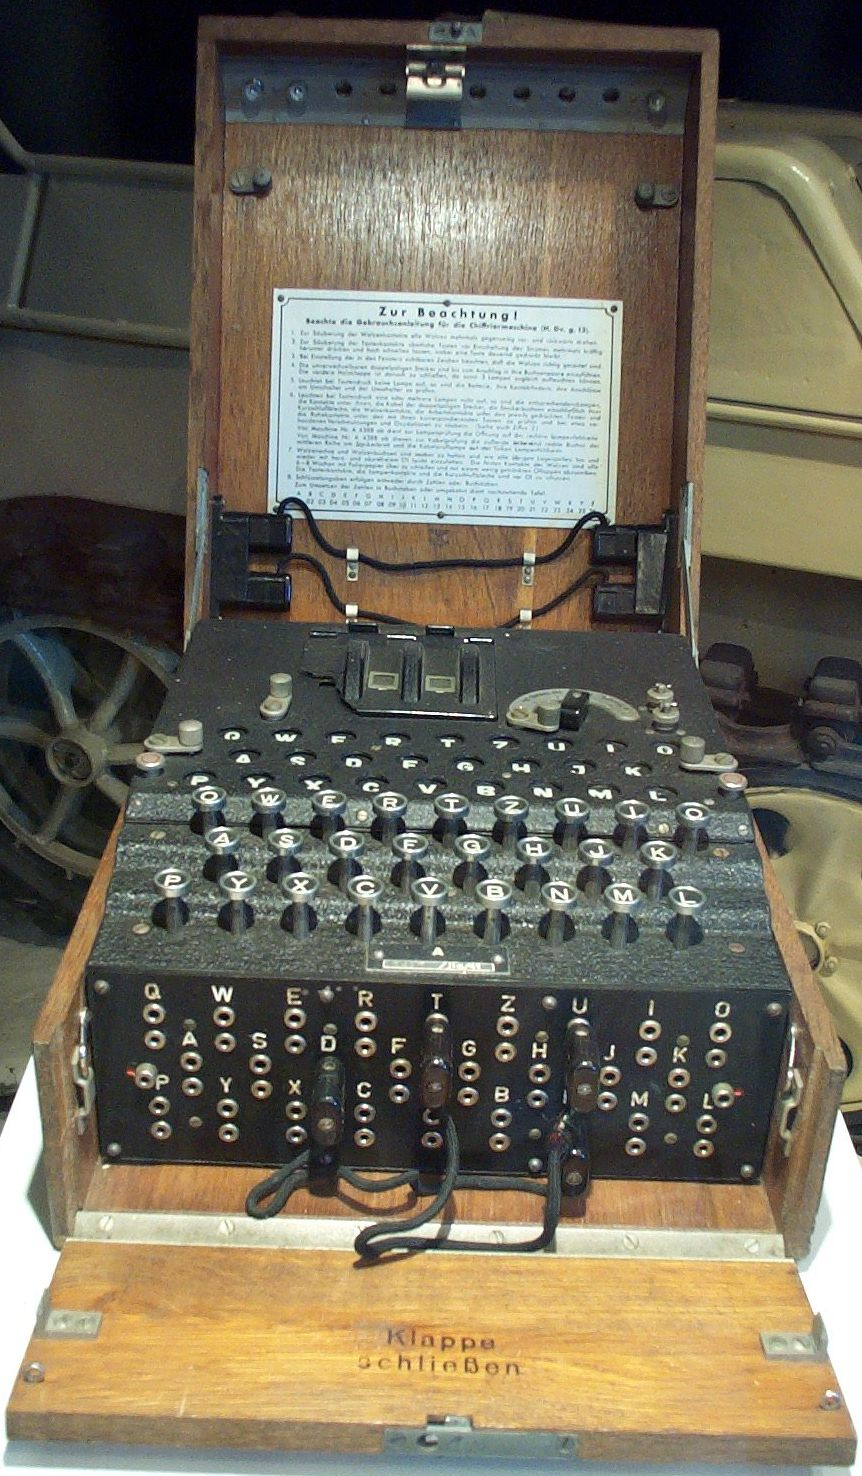
\includegraphics[width=5cm]{images/Enigma_Verkehrshaus_Luzern_cropped.jpg}
\caption{Enigma Maschine}
\end{center}
\end{figure}

\subsubsection{Funktion der ENIGMA Maschine}
Die Walzen können sich drehen und sind mit Elektrischen Kontakten miteinander verbunden. Wird eine Taste gedrückt, fliesst Strom durch den Walzenssatz und es leuchtet die Lampe des verschlüsselten Buchstabens auf. Die Walze dreht sich bei jedem Tastendruck weiter, so das der gleiche Buchstaben jeweils anders verschlüsselt wird. Z. B. AAA wird zu DEF. Nach 26 Umdrehungen der ersten Walze wird die zweite Walze gedreht. \\

\begin{figure}[ht]
\begin{center}
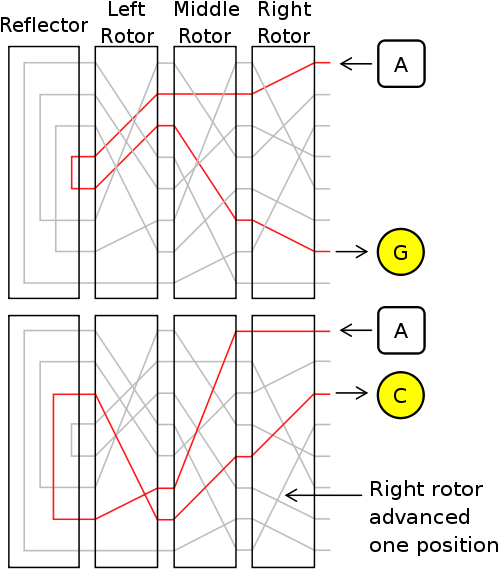
\includegraphics[width=5cm]{images/Enigma-action.png}
\caption{Enigma Stromfluss}
\end{center}
\end{figure}

Dabei gehen jeweils elektrische Impulse durch die Walze. Nach jeder Drehung legt der Strom eine andere Strecke durch die Walzen zurück. 
Über das Steckbrett konnte der Verschlüsselte Buchstaben nochmals ersetzt werden. z. B. wurde E mit J verbunden. Falls nach dem verschlüsseln ein E herauskam, wurde dieses mit J ersetzt. 

\subsubsection{Anwendung}
Die Deutsche Wehrmacht nutzte die ENIGMA um ihre Funksprüche zu verschlüsseln. Dazu wurden jeweils um Mitternacht die Walzen und die Steckverbindungen ausgetauscht bzw. umgesteckt. Ein neuer Schlüsselsatz sah beispielsweise so aus:

%Quelle Wikipedia%
\begin{table}[ht]
\caption{Schlüsseltafel der Wehrmacht}
\begin{center}
\begin{tabular}{|l|l|l|l|l}
Tag & UKW & Walzenlage & Ringstellung &  ---- Steckerverbindungen ---- \\
 31  &   B   &  I   IV III   &    16 26 08   &  AD CN ET FL GI JV KZ PU QY WX \\
\end{tabular}
\end{center}
\end{table}

Die eigentliche Verschlüsselung war relativ simpel zu bewerkstelligen. Es musste nur die entsprechende Funknachricht eingegeben werden und die ENIGMA erledigte die Verschlüsselung. Der Austausch der aktuellen Walzenstellung und das Morsen der Nachricht waren jedoch wesentlich komplizierter.

Vor der Eigentlichen Nachricht wurde ein Nachrichtenkopf gemorst. In diesem wurde die länge des Textes bekannt gegeben, die Walzenstellung und die Nachrichtenart. 
Der eigentliche Text wurde in Gruppen aus 5 Buchstaben gemorst. Bei den ersten 5 Buchstaben wurde bestimmt, an wenn die Nachricht geht. Dabei wurden die ersten zwei Buchstaben zufällig ausgewählt und die letzten 3 durchmischt. Nach der Alphabetischen Ordnung, konnte über eine Tabelle festgestellt werden, ob die Nachricht einem was angeht, bevor man sie entschlüsselt.
Die Walzenstellung wurde ebenfalls nicht einfach übertragen. Wenn im Kopf z. B. QWE EWG angegeben wurde, hiess das man soll die Walze auf die Buchstaben QWE einstellen und EWG eingeben. Was dabei verschlüsselt heraus kam, war die Anfangsstellung der Walzen. Jetzt konnte mit der Decodierung der Nachricht begonnen werden.

\subsubsection{Schwachstelle der ENIGMA}
Die Enigma benutzte ein Symetrisches Verfahren, wobei die Verschlüsselung und Entschlüsselung gleich sind. %Siehe Kapitel Symetrische Verfahren%
Die Geheimhaltung der Walzen war wichtig, da sie einen wesentlichen Teil der Verschlüsselung ausmachen.
Dadurch das ein Buchstabe nicht in sich selbst verschlüsselt werden kann (Strom kann nicht zurück fliessen) konnte ein wesentlicher Teil ausgeschlossen werden.
Durch einsetzen bestimmter Wörter, welche im Text vermutet wurden, konnte ein grosser Teil der möglichen Positionen ausgeschlossen werden. Dafür wurde z. B. OBERKOMMANDODERWEHRMACHT eingesetzt und falls an einer Position der Buchstabe in sich selbst verschlüsselt war, konnte das Wort an dieser Position nicht sein.

\subsection{Probleme der früheren Verschlüsselungen}
Die Verfahren bis zum zweiten Weltkrieg konnten einfach geknackt werden. Wenn die Art der Verschlüsselung bekannt war, konnte der Schlüssel einfach ermittelt werden. 
Die Enigma revolutionierte die Kryptographie. Obwohl die Art der Verschlüsselung und sogar die Walzen bekannt waren, mussten die Engländer grosse Anstrengungen unternehmen, damit die Texte entschlüsselt werden konnten. Um der Enigma zu begegnen wurden Maschinen gebaut, welche diese Arbeit vereinfachten. Die sogannte Turing Bombe konnte innert 6 Stunden die Verschlüsselung knacken. 
Mit mehreren Turing Bomben wurde die Verschlüsselung in vernüfntiger Zeit geknackt. \\

Die früheren Verschlüsselungen hielten sich nicht an das Kerckhoff's Prinzip. Dieses besagt, das die Sicherhiet der Verschlüsselung nicht von der Geheimhaltung des Algorithmus abhängig gemacht werden darf. Die Sicherheit ist durch den Schlüssel gegeben. 
\newpage
\section{Moderne Kryptographie}
Dieses Kapitel wurde mit Hilfe des Buches \textit{Moderne Verfahren der Kryptographie} erarbeitet.\\[2ex]
Die moderne Kryptographie unterscheidet sich von der klassischen Kryptographie in der Technik. Was früher mechanisch errechnet wurde, wird in der modernen Kryptographie elektronisch erledigt. Mit dieser technischen Hilfe ist es möglich, komplexe Berechnungen in vernünftiger Zeit durchzuführen. Die grossen Chiffriermaschienen werden durch den Computer abgelöst.\\
Die immer besseren, beziehungsweise schnelleren Computer machen die klassische Kryptographie sehr unsicher, da der Schlüssel durch Brute-Force-Angriffe\footnote{Brute-Force nennt man dass Vorgehen, ein Passwort durch Ausprobieren aller möglichen Schlüssel zu knacken.} schnell gefunden werden kann.\\
Man brauchte also sichere Verschlüssselungs-Methoden, die durch Ausprobieren nicht geknackt werden konnten.\\
Einen grossen Fortschritt machte die moderne Krypographie in den Jahren 1976 und 1985.\\
% TODO ZERO-KNOWLEDGGE Verweis
1976 wurde das Problem, dass immer beide Seiten einen \textbf{gemeinsamen} Schlüssel benötigen gelöst. Das ist die Geburtstunde des RSA-Algorithmus.\\
1985 entwickelten drei Mathematiker/-Innen das \textbf{Zero-Knowledge-Verfahren}. \cite{} Das Zero-Knowlede-Verfahren baut auf dem RSA-Algorithmus auf und Unterscheidet sich in der Implementierung des Protokols. Mit diesem Verfahren ist es möglich, dass zwei Personen auf einem Rechner miteinander kommunizieren, ohne dass der Rechner davon etwas erfährt.
%
\subsection{Symmetrische Verschlüsselung}
Grundsätzlich braucht es für eine einfache symmetrische Verschlüsselung einen Schlüssel, den zu verschlüsselten Text und eine Verschlüsselungsfunktion.
Die Verschlüsselungsfunktion übersetzt den Klartext mit Hilfe des Schlüssel. In einer Formel ausgedrückt:
\begin{equation*}
  c = f ( k, m )
\label{eqn:sym_versch}
\end{equation*}
\textit{c} steht für den verschlüsselten  (eng.: \textit{crypted}) Text, \textit{f} für die Verschlüsselungsfunktion (eng.: \textit{function}), \textit{k} für den Schlüssel (eng.: \textit{key}) und \textit{m} für den Text (eng.: \textit{message}) den man verschlüsseln möchte.\\
%
Der verschlüsselte Text wird nun dem Empfänger übergeben. Hat der Empfänger keinen Schlüssel \textit{k}, um die Nachricht zu entschlüsseln, kann er die Nachricht nicht lesen. Somit braucht der Empfänger \textbf{denselben} Schlüssel \textit{k}, die verschlüsselte Nachricht \textit{c} und eine Umkehrfunktion von \textit{f}.\\
Daraus ensteht die Formel:
\begin{equation*}
  m = f^*(k ,c)
\label{eqn:sym_entsch}
\end{equation*}
%Kerckoff's Prinzip bei  Schwachstellen DENIS
Man geht davon aus, dass die Funktionen der Ver- und Entschlüsslung öffentlich bekannt sind, was überraschenderweise kein Sicherheitsproblem darstellt. Aus dem Kerckhoffs' Prinzip geht der Grundsatz hervor, dass die Sicherheit eines Verschlüsslungsverfahren nicht auf der Geheimhaltung des Algorithmus, sondern auf die Geheimhaltung des Schlüssels beruht, denn ein Algorithmus kann durch Reverse-Engineering\footnote{Unter dem Begriff Reverse-Engineering versteht man den Vorgang, aus einem fertigen Produkt durch Untersuchung der Strukturen und Verhaltensweisen den Source Code herauszufinden.} rekonstruiert werden.\\
Auch hat die Geschichte gezeigt, dass bis heute viele Verschlüsselungsalgorithmus gebrochen werden konnte. \cite{mod_kry}\\
%
Somit muss die Verschlüsselungsfunktion so komplex sein, dass man nur mit dem Schlüssel das richtige Ergebnis erhält.
%
%******************************************
%  Asymetrische Verschlüsselung
%******************************************
\subsection{Asymmetrische Verschlüsselung}
Vor 1970 als es die asymmetrische Verschlüsselung noch nicht gab, wurden Schlüssel für eine symmetrische Verschlüsselung unter grossem Schutz transportiert.
%
Es waren vor allem die Botschaften, die einen solchen Transport mehrfach absicherten, indem sie dem Überbringer den Koffer mit Handschellen am Handgelenk festmachten und ihn von diversen Bodyguards beschützt in einer panzerfesten Limousine zum Zielort fuhren.\\
Dieses Verfahren war sehr umständlich. Es kostete viel und dauerte zu lang. Wie aber sollte man einen Schlüssel sicher von einem Ort zum andern transportieren und dabei sicher sein, dass niemand einen Blick auf den Schlüssel werfen konnte?\\
%
Anfang 1976 stellten Whitfield Diffe und Martin Hellman ein Konzept vor, das die Grundidee von einer asymmetrischen Verschlüsselung darlegte. Sie kannten das Verfahren jedoch nicht exakt. Sie stellten das \textbf{Diffle-Hellman-Problem} vor. \cite{rsa_and_public_key}\\ % Stellten das Prinzip vor
Schon viel früher entwickelten James Ellis, Clifford Cockes und Malcom Willamson, alle vom Britischen Geheimdienst, ein asymmetrisches Verschlüsselungsverfahren. Sie durften aber ihre Ergebnisse weder veröffentlichen noch ein Patent anmelden. 
Der Erfolg gelang Ronald L. \textbf{R}ivest, Adi \textbf{S}hamir und Leonard M. \textbf{A}dleman im Jahre 1977. Sie entwickelten den RSA-Algorithmus, der bis heute als einer der sichersten asymmetrischen Verfahren gilt.\\[2ex]
%
Bei einem asymetrischen Verfahren kann der Sender dem Empfänger eine verschlüsselte Nachricht senden, die nur der Empfänger entschlüsseln kann.\\
%
Das funktioniert dank einem öffentlichen Schlüssel, dem \textbf{Public-Key}, und einem privaten Schlüssel, dem \textbf{Private-Key}. Beide zusammen bilden das Schlüsselpaar.\\
Für dieses Verfahren hat sich der Name \textbf{Public Key-Kryptographie} durchgesetzt.
%
% Bei der Formel für die verschlüsselung ist f_e und m verantwortlich für c das heisst es sind beide wichtig!!
%
Um jemandem eine verschlüsste Nachricht zu senden, benötigt man den öffentlichen Schlüssel des Empfängers. Mit diesem öffentlichen Schlüssel und der Verschlüsselungsfunktion wird der Klartext in ein Chiffrat übersetzt. Nur der Besitzer des pirvaten Schlüssels ist in der Lage, aus dem Chiffrat den Klartext zu erzeugen.\\
Die Verschlüsselung in einer Formel ausgedrückt:\\
%Aus dieser Idee kann man eine Funktion erstellen, die das Verschlüssen schematisch darstellt.\\
\begin{equation*}
  c = f_e (m)
  \label{eqn:asy_versch}
\end{equation*}
Der Verschlüsselungsalgorithmus \textit{f} verschlüsselt den Klartext \textit{m} in den verschlüsselten Text \textit{c} mit Hilfe des öffentlichen Schlüssels \textit{e} (eng.: \textit{encription exponent}).\\
% c = f(e,m)
%\paragraph{Entschlüsseln}
%Der Empfänger empfängt den verschlüsselten Text und entschlüsselt ihn mit Hilfe seines privaten Schlüssel und erhält den Klartext.
%Auch hier läst sich dieses Vorgehen in einer Funktion beschreiben.\\
%Mit der Entschlüsselungsfunktion f und dem privaten Schlüssel d wird aus dem verschlüsseltem Text c den Klartext m' gewonnen.
Die Entschlüsselung in einer Formel ausgedrückt:
\begin{equation*}
  m' = f_d (c) 
  \label{eqn:asy_entsch}
\end{equation*}
Mit der Entschlüsselungsfunktion \textit{f} und dem privaten Schlüssel \textit{d} (eng.: \textit{decription exponent}) wird aus dem verschlüsseltem Text \textit{c} den Klartext \textit{m'} gewonnen.
%
Das Wichtigste bei der asymmetrischen Verschlüsselung ist, dass beim Entschlüsseln wieder der \textbf{gleiche} Text reproduziert wird, auch wenn zum Ver- und Entschlüsseln zwei unterschiedliche Schlüssel verwendet wurden.\\
Der ganze Vorgang in einer Gleichung ausgedrückt (c parametrisiert):
\begin{equation*}
  m' = f_d (c) = f_d (f_e (m) ) = m \\
  \label{eqn:asy_togh}
\end{equation*}
gekürzt\\
\begin{equation*}
  m = f_d ( f_e (m) )
  \label{eqn:asy_togh_shortForm}
\end{equation*}
%\paragraph{Beispiel \footnotemark}
%Herr Müller möchte gern Herrn Spinnler seine sensiblen Daten übergeben. Dafür benötigt er den öffentlichen Schlüssel von Herr Spinnler.\\
%Jetzt verschlüsselt Herr Müller mit dem öffentlichen Schlüssel seine Daten und sendet das Paket an Herrn Spinnler. Dieser wiederum entschlüsselt das Paket mit seinem geheimen, gut aufbewarten, privaten Schlüssel. Jetzt ist er im Stande die Nachricht von Herrn Müller zu lesen.

%\footnotetext{Dieses Beispiel zeigt einen schematischen Ablauf. Es geht nicht auf das Verschlüsselungsverfahren ein.}
% Erwähnen dass man bei der Asymetrischen Verschlüsselung Einwegfunktionen benötigt

%Im wirklichkeit sieht das Verfahren so aus. Eine Person A erstellt zwei Schlüssel. Einen privaten Schlüssel, der nur sie kennt und einen öffentlichen, d%en sie Person B gibt. Jetzt möchte B an A einen Text senden. Hierfür nimmt es den öffentichen Schlüssel von A und verschlüsselt den Text.
%Diesen Verschlüsselten Text sendet Person B an A. 
%A nimmt jetzt den verschlüsselten Text entgegen und entschlüsselt ihn mit Hilfe des privaten Schlüssel.
%Da A nur den privaten Schlüssel hat, mit der sich den verschlüsselten Text entschlüsseln lässt, kann nur A den Text lesen.
%Der Empfänger erstellt zwei Schlüssel. Einen öffentlichen den er verteilen kann und einen geheimen privaten Schlüssel denn er keinem zeigt. 

%
%-----------------------------------------------------------
%RSA-Algorithmus erklären anhand von Beispielen
%-----------------------------------------------------------
\newpage
\part{Der RSA-Algorithmus}
\section{Mathematisches Verfahren}
Dieses Kapitel wurde mit Hilfe des Buches \textit{Moderne Verfahren der Kryptographie}\cite{mod_kry}, \textit{Zahlentheorie für Einsteiger}\cite{zahlentheorie_fuer_einsteiger} und \textit{Kryptologie}\cite{kryptologie} erarbeitet.\\[2ex]
%
Der RSA-Algorithmus baut grundsätzlich auf Primzahlen, der Modulo und Eulerschen-Funktion, dem Satz von Euler und dem erweiterten euklidischen Algorithmus auf.\\
Im nächsten Abschnitt werden die einzelnen mathematischen Verfahren kurz in ihren Funktionen erläutert.\\
Wir werden für die beiden Primzahlen durchgehend die Variablen $p$ und $q$ verwenden. $N$ steht immer für das Produkt von $p \cdot q$. Die Variable $r$ wird für das Resultat der Modulo-Berechnungen verwendet. $e$ steht für den Verschlüsselungs-Exponenten und $d$ für den Entschlüsselungs-Exponenten.
%
\subsection{Modulo}
Modulo oder auch \textit{Division mit Rest} gibt den ganzzahligen Rest einer Division zweier natürlichen Zahlen an. Er wird beim RSA-Algorithmus bei der Berechnung des Entschlüsselungs-Exponenten sowie in der Verschlüsselung verwendet.\\
Modulo erklärt sich am Einfachsten an einem Beispiel:
%
\begin{equation*}
  21 \bmod(5) = 1
\end{equation*}
%
Es gilt herauszufinden, wie viel Mal 5 ganz in 21 vorhanden ist. Dafür teilen wir 21 durch 5 und schneiden den Dezimalrest ab. Um den ganzzahligen Rest zu berechnen subtrahieren wir von 21 das Produkt aus 4 mal 5.
%
\begin{flalign*}
  21 \colon 5 &= 4.2\\
  21 - 4 \cdot 5 &= 1\\
  21 &= 4 \cdot 5 + 1
\end{flalign*}
%Oder für den RSA Algorithmus veralgemeinert:
%\begin{equation}
%  \varphi(N) = q \cdot e + r
%  \label{eqn:mod_rsa}
%\end{equation}
%
\paragraph{Kongruent Modulo}
Kongruent Modulo bedeutet nichts anders, als dass zwei verschiedene Zahlen Modulo einer gleichen Zahl den selben Rest haben. Man sagt auch, dass sie in der gleichen Restklasse sind.\\
Als Beispiel nehmen wir die Zahlen 9 und 7 die Modulo 2 gerechnet werden.
%
\begin{flalign*}
  9 \bmod(2) &= 1 \\
  7 \bmod(2) &= 1  \\
  9 & \equiv 7 \bmod(2)
\end{flalign*}
%
%******************************************************************************
% Eulersche Funktion
%******************************************************************************
%Verbessern die Zahlen sind kleiner als die Zahl
\subsection{Eulersche Funktion}

Die Eulersche Funktion zählt die natürlichen, teilerfremden\footnote{Zwei Zahlen sind teilerfremd zueinander, wenn ihr grösster gemeinsamer Teiler 1 ist.}  Zahlen von n, die kleiner als n sind.\\
Für die Eulersche Funktion stellen die Primzahlen einen Spezialfall dar.
Primzahlen sind nur durch 1 und sich selbst ohne Rest teilbar. Somit ist das Resultat der die Eulerschen Funktion einer Primzahl p immer $p - 1$.\\
Um den privaten Schlüssel zu errechnen, muss man $\varphi(N)$ beziehungsweise $\varphi(pq)$ berechnen. Aus diesem Grund erläutern wir die Eulersche Funktion:
%
\begin{equation*}
  \varphi(p) = p - 1
\end{equation*}
%
Der grösste gemeinsame Teiler zweier Primzahlen ist immer 1.
Für die Eulersche Funktion zweier Primzahlen gilt:
\begin{equation}
  \varphi(pq) = \varphi(p) \cdot \varphi(q) = (p - 1) \cdot (q - 1)
  \label{eqn:eulersche_func}
\end{equation}
Der Beweis dafür liefert folgende Überlegung. Es gibt insgesamt $p \cdot q -1$ ganze Zahlen die kleiner sind als $p \cdot q$.\\
Es ist bei Primzahlen einfacher, die \textbf{nicht teilerfremden} Zahlen zu zählen und diese dann von allen möglichen Zahlen abzuziehen, als alle teilerfremden Zahlen zu zählen. Nicht teilerfremd zu p sind $(q - 1) \cdot p$ und für q gilt $ (p - 1) \cdot q$. \cite{kryptologie}\\
Als Formel geschrieben:
%
\begin{equation*}
  \begin{split}
    \varphi(pq) & = p \cdot q -1 - (p - 1) - (q - 1)  \\
     & = p \cdot q -1 - p + 1 - q + 1  \\
     & = p \cdot q -q - p + 1  \\
     & = (p -1) \cdot (q - 1)
    \label{eqn:herleitung_eulersche_func}
  \end{split}
\end{equation*}
%
% Satz von Euler
%=====================
%Verweis auf Buch Beutelspacher
\subsection{Satz von Euler}
Der Satz von Euler gewährleistet die korrekte Ver- und Entschlüsselung.\cite{zahlentheorie_fuer_einsteiger}. Wir gehen hier nicht weiter auf den Satz von Euler ein und werden später beim Beweis nochmals auf ihn zurückkommen.\\
Der Satz von Euler sagt über zwei natürliche, teilerfremde Zahlen, hier $n$ und $m$, folgendes aus: \cite{kryptologie}
%
\begin{equation}
  m^{\varphi(n)} \bmod(n) = 1
  \label{eqn:satz_von_euler}
\end{equation}
%
Nehmen wir für $n = 15$ und $m = 4$ und setzen Formel [\ref{eqn:satz_von_euler}] ein.
%
% Zeigen das varphi 15 = 8 ist
\begin{flalign*}
  4^{\varphi(15)} \bmod(15) = 1  \\
  4^8 \bmod(15) = 1
\end{flalign*}
%
%
% Kleiner Satz von Verma
%
%Wenn wir jetzt eine natürliche Zahl k nehmen, gilt für diese folgende Gleichung (Erleuterung siehe Buch \textit{Kryptologie}):
%
%\begin{equation}
%  \begin{split}
%    m^{1 + k \cdot \varphi(N)} \bmod(N)  &= m \cdot 1 \\
%    m \cdot m^{k \cdot \varphi(N)} \bmod(N) &= m \cdot 1
%    \label{eqn:satz_von_euler_erweitert}
%  \end{split}
%\end{equation}
%
%
%Hat man zwei verschiedene Primzahlen p und q und eine natürliche Zahl m, die kleiner ist als $p \cdot q$, dann gilt für jede natürliche Zahl k:
%
%\begin{equation}
%  m^{k \cdot (p - 1) \cdot (q - 1) +1} \bmod(p \cdot q) = m
%  \label{eqn:kleiner_satz_fermat}
%\end{equation}
%
%Dieser Satz wird in der Mathematik auch \textit{kleiner Satz von Fermat} genannt.
% Buch S 109 / 110
%
%******************************************************************************
% Euklidischer Algorithmus
%******************************************************************************
\subsection{Euklidischer Algorithmus}\label{euklidischer_Algorithmus}
Mit den Euklidischen Algorithmen lässt sich der grösste gemeinsame Teiler (ggT) zweier natürlichen Zahlen berechnen. Es existiert das etwas ältere Subtraktionsverfahren und das moderne Modulo-Verfahren. Da das Subtraktions-Verfahren nicht die gleiche Effizienz hat wie das Subtraktionsverfahren, konzentrieren wir uns auf das Modulo-Verfahren. \cite{zahlentheorie_fuer_einsteiger}\\
Für den RSA-Algorithmus ist es wichtig, dass wir zwei teilerfremde Zahlen $\varphi(N)$ und $e$ haben.\\
%
Die Formel für das Modulo-Verfahren lautet:
%
\begin{equation}
  \label{eqn:euklidischer_algo}
  a = b \cdot q + r 
\end{equation}
%
wobei
\begin{equation*}
  0 \leq r \leq e - 1
\end{equation*}
gelten.\\
%
Auf den RSA-Algorithmus bezogen sieht die Formel so aus:
\begin{equation}
  \label{eqn:euklidischer_algo_RSA}
  \varphi(N) = q \cdot e + r 
\end{equation}
%
Dabei sind $\varphi(N)$ und e die beiden Zahlen von denen wir den grössten gemeinsamen Teiler ausrechnen.
Wir gehen davon aus das $\varphi(N)$ grösser ist als e. Wäre das nicht der Fall, müsste e auf die linke Seite des Gleichheitszeichen.
Zur Veranschaulichung nehmen wir zwei Zahlen $\varphi(N) = 839$ und $e = 199$ und setzen diese in unsere Gleichung ein.
\begin{enumerate}
  \item Schritt: Zahlen in Gleichung einsetzen, q und r ausrechnen.\\
    \begin{equation*}
      839 = 4 \cdot 199 + 43
    \end{equation*}
  \item Schritt: 199 als neues $\varphi(N)$ und 43 als neues e einsetzten und wieder q und r ausrechnen.\\
    \begin{equation*}
      199 = 4 \cdot 43 + 27
    \end{equation*}
\end{enumerate}
Den zweiten Schritt solange wiederholen bis man auf Rest 1 oder 0 kommt. Falls die Zahl 0 herauskommt, nehmen wir den Rest der vorangegangenen Gleichung als grössten gemeinsamen Teiler.\\
%
Ganzer Ablauf:
\begin{equation*}
  \begin{split}
    839 &= 4 \cdot 199 + 43\\
    199 &= 4 \cdot 43 + 27\\
    43 &= 1 \cdot 27 + 16\\
    27 &= 1 \cdot 16 + 11\\
    16 &= 1 \cdot 11 + 5\\
    11 &= 2 \cdot 5 + 1\\
    \label{eqn:euqulid_beweis}
  \end{split}
\end{equation*}
%
Der grösste gemeinsame Teiler von 839 und 199 ist 1. Sie sind daher teilerfremd. \\[2ex]
Um dieses Verfahren zu beweisen, gehen wir davon aus, dass $\varphi(N)$, e, r und q alles natürliche nicht negative Zahlen sind. Da wir im zweiten Schritt den grössten gemeinsamen Teiler von $e$ und r errechnet haben, kann man basierend auf Formel \ref{eqn:euklidischer_algo_RSA} folgende Behauptung aufstellen:
%
\begin{equation}
  ggT(\varphi(N),e) = ggT(e,r)
  \label{eqn:ggT}
\end{equation}
%
Nur der grösste gemeinsame Teiler von $\varphi(N)$ und $e$ teilt sowohl $\varphi(N)$ als auch e und r ohne Rest. Auf unser Beispiel angewendet ergibt das $ggT(839,199) \leq ggT(199,43)$.\\
Und es gilt: Nur der grösste gemeinsame Teiler von e und r teilt auch $\varphi(N)$ ohne Rest.\\
Das heisst: $ggT(199,43) \leq ggT(839,199)$.
Somit stimmen die beiden grössten gemeinsamen Teiler überein\cite{zahlentheorie_fuer_einsteiger}.\\[2ex]
Gehen wir zurück zu unserem Beispiel:
%
\begin{equation*}
 ggT(839,199) = ggT(199,43) = ggT(43,27) = ggT(27,16) = ggT(16,11) = ggT(11,5) = 1
\end{equation*}
%
%******************************************************************************
% Erweiterter Euklidischer Algorithmus
%******************************************************************************
\subsubsection{Erweiterter Euklidischer Algorithmus}
Der erweiterte Euklidische Algorithmus berechnet neben dem grössten gemeinsamen Teiler $r$ zweier natürlichen Zahlen auch noch die dazugehörigen natürlichen Zahlen d und k, dass folgende Gleichung stimmt:
%
\begin{equation}
  ggT(a,b) = s \cdot a + t \cdot b
  \label{eqn:erw_euklid_algo}
\end{equation}
%
Auf den RSA-Algorithmus angewendet sieht die Formel so aus:
%
\begin{equation}
  r = d \cdot e + k \cdot \varphi(N) 
  \label{eqn:erw_euklid_algo_RSA}
\end{equation}
%
Mit seiner Hilfe lässt sich der Entschlüsselungs-Exponent d berechnen, welchen wir für die Berechnung des privaten Schlüssels brauchen.\\
Dieser Algorithmus wird auch \textit{Vielfachsummendarstellung} genannt, denn um auf die Zahlen d und k zu kommen, muss man die Vielfachsummendarstellung anwenden.\\
Es ist eine erweiterte Form des Euklidischen Algorithmus.\\
Wir schreiben jetzt die Rechnung \ref{eqn:euqulid_beweis} so um, dass wir den Rest auf einer Seite isolieren.\\ 
\begin{equation}
  r = \varphi(N) - a \cdot e
  \label{eqn:form_erw_euklid}
\end{equation}
%
\begin{flalign*}
  43 &= 839 - 4 \cdot 199\\
  27 &= 199 - 4 \cdot 43\\
  16 &= 43 - 1 \cdot 27\\
  11 &= 27 - 1 \cdot 16\\
  5 &= 16 - 1 \cdot 11\\
  1 &= 11 - 2 \cdot 5
  \label{eqn:erw_euklid_10}
\end{flalign*}
%
% TODO: AUSSCHREIBEN
Man startet bei der untersten Zeile und ersetzt die Zahl, die den nächsten oberen Rest beschreibt, durch die Gleichung. Das heisst man ersetzt in der ersten Gleichung die Zahl $5$ mit dem Term $16 - 1 \cdot 11$. Das wiederholt man so lange, bis man die letzte Gleichung eingesetzt hat. 
Es ist zu beachten, dass auf der rechten Seite eine Summe aus zwei Produkten stehen bleibt.
%
\begin{flalign*}
  1  &= 11 - 2 \cdot 5 = 11 - 2 \cdot 16 + 2 \cdot 11 = 3 \cdot 11 - 2 \cdot 16 \\
  &= 3 \cdot 11 - 2 \cdot 16 = 3 \cdot 27 - 3 \cdot 1 \cdot 16 - 2 \cdot 16 = 3 \cdot 27 - 5 \cdot 16\\
  &= 3 \cdot 27 - 5 \cdot 16 = 3 \cdot 27 - 5 \cdot 43 + 5 \cdot 1 \cdot 27 = 8 \cdot 27 - 5 \cdot 43\\
  &= 8 \cdot 27 - 5 \cdot 43 = 8 \cdot 199 - 8 \cdot 4 \cdot 43 - 5 \cdot 43 = 8 \cdot 199 - 37 \cdot 43\\
  &= 8 \cdot 199 - 37 \cdot 43 = 8 \cdot 199 - 37 \cdot 839 + 37 \cdot 4 \cdot 199 = 156 \cdot 199 - 37 \cdot 839
\end{flalign*}
%
Am Schluss bekommen wir die Formel
%
\begin{equation*}
 1 = 156 \cdot 199 + (-37) \cdot 839
 \label{eqn:erw_euklid_end}
\end{equation*}
%
Damit wir jetzt den Entschlüsselungs-Exponenten d bekommen, müssen wir die Gleichung in die Modulare Inverse umschreiben. Wir berechnen somit die Modulare Inverse von $\varphi(N)$ und e.\\
Die Formel der modularen Inverse auf den RSA-Algorithmus angewendet lautet:
\begin{equation}
  e \cdot d \bmod(\varphi(N)) \equiv 1
\end{equation}
%
Wir gehen von Formel \ref{eqn:erw_euklid_end} aus und setzen den Term $(-37) \cdot 839$ auf die linke Seite.
%
\begin{equation*}
 1 - 37 \cdot 839 = 156 \cdot 199
\end{equation*}
Damit man den nächsten Schritt versteht, muss man wissen, dass man eine Gleichung
\begin{equation*}
  1 + k \cdot \varphi(N) = d \cdot e
\end{equation*}
mit Modulo ausdrücken kann.
\begin{equation*}
  1 \equiv d \cdot e \bmod(\varphi(N))
  \label{eqn:erw_eukl_fertig}
\end{equation*}
%
Aufgrund dessen können wir die Modulare Inverse von $\varphi(N)$ und e so ausdrücken:
%
\begin{equation*}
 1 \equiv 156 \cdot 199 \bmod(839)
\end{equation*}
Wir erhalten den Entschlüsselungs-Exponent $d = 156$.
%
%Um das zu beweisen schauen wir uns nochmal die Formel \ref{eqn:euklidischer_algo} an. Aus einer Vielfachsummendarstellung von $q$ und $r$, lässt sich dei Vielfachsummendarstellung von $p$ und $q$ ableiten. Man kann die Formel
%{eqn:ggT}
%\begin{equation*}
%  2 = x \cdot p + y \cdot q
%  \label{eqn:erw_eukl_fertig}
%\end{equation*}
%
%auch mit r und a darstellen.
%
%\begin{equation*}
%  2 = x \cdot r + y \cdot a
%\end{equation*}
%
%Jetzt setzen wir die Formel \ref{eqn:form_erw_euklid} anstatt r ein und erhalten diese Gleichung
%\begin{equation*}
%  2 = x \cdot (p - a \cdot q)  + y \cdot a = x \cdot p + (y - xa) \cdot q
%\end{equation*}
%
%Somit haben wie die Vielfachsummendarstellung für $p$ und $q$.
%
%\subsubsection{Modulare Inverse}
%Haben wir zwei natürliche, teilerfremde Zahlen, gibt es eine Zahl x, sodass die Formel
%
%\begin{equation*}
%  p \cdot x \bmod(q) \equiv 1
%\end{equation*}
%
%Es gibt zwei ganze Zahlen $x$ und $y$ sodass die Gleichung \ref{eqn:erw_eukl_fertig} entsteht.
%Weil $y cdot q$ durch $q$ teilbar ist, gibt es bei der Divison von $x \cdot p$ durch $q$ immer 1. Somit kann man sagen
%
%\begin{equation}
%  p \cdot x \bmod q = 1
%  \label{eqn:mod_inverse}
%\end{equation}
%
%Die Modulareinverse von zwei teilerfremden natürlichen Zahlen $p$ und $q$, errechnet man mit dem erweiterten Euklidischen Algorithmus. Dann ist $x$ die modulare Inverse von $p$ und $q$.


\section{Der Schlüssel}
Für eine sichere Verschlüsslung kommt es auf den Schlüssel an. Denn nur mit diesem Schlüssel, kann man die verschlüsselte Nachricht enschlüsseln. Der Schlüssel spielt also eine zentrale Rolle und muss sicher sein.

\subsection{Sicherer Schlüssel generieren}
Für einen sicheren Schlüssel sollte man immer Zufallszahlen verwenden. Zufallszahlen sind Zahlenfolgen bei denen man die nächste Zahl nicht durch mathematische Berechunungen vorhersagen kann - also Zufällige Zahlen. 
\subsubsection{Zufallszahlen generieren}
Um solche Zufallszahlen zu generieren hat man Zufallszahlengeneratoren (engl random number generator = RNG) gebaut. Diese messten den Radioaktiven Zerfall oder beobachteten die atmosphärischen Bedingungen in der Umgebung. Die Zahlen die der RNG zurückgibt, kann man dann Verwenden um eine Zufallszahl zu generieren, da der Output auf einem Input basiert, der sich permanent ändert und nicht wiederholbar ist.

Was, wenn man keine solchen Messgeräte hat, die solche Zahlen generieren können. 
Für das gibt es Pseudozufallszahlengeneratoren (engl pseudo random number generator = PRNG)

\paragraph{Entropie}
\paragraph{Zahlentheoretische Funktionen}
\subsection{Schlüssel austauschen}

\section{RSA Verschlüsselung}
Die RSA Verschlüsselung wurde 1977 von Ronald L. Riverst, Adi Shamir und Leonard Adleman entwickelt. Der Name RSA setzt sich aus den Anfangsbuchstaben der Nachnamen der Entwickler zusammen. Es handelt sich um ein asymmetrisches Verfahren. (Siehe Kapitel moderne Kryptographie) %Verweis%
Das RSA Verfahren wird auch heute noch oft eingesetzt. Das Verfahren gilt bei einer bestimmten Schlüssellänge als sicher. Es gibt verschiedenste Angriffsmöglichkeiten, diese führen jedoch nicht in einem vernünftigen Zeitraum zu Ergebnissen. Das Verfahren wird zur Signierung und zur Verschlüsselung verwendet. (Siehe Anwendung) %Verweis%

\subsection{Formel Verschlüsselung}
Wenn der Schlüssel erstellt wurde kann ein Text einfach verschlüsselt werden. Dazu dient folgende Formel:
$ C \equiv m^e  \bmod N $\\
C steht für Cipher und bezeichnet den Geheimtext. Dieser ist abhängig von der Nachricht m, dem öffentlichen Schlüssel e und dem RSA-Modul N.

\section{RSA Entschlüsselung}
Die RSA Entschlüsselung ist ohne den Geheimschlüssel zu wissen nicht möglich. Da die Sicherheit von diesem Geheimschlüssel abhängt, gilt es diesen möglichst lang zu wählen und geheim zu halten. Aktuell gilt eine Schlüssellänge von 2048 Bit als sicher. Als Dezimalzahl ausgedrückt, ist dies eine Zahl von $ 3,2 * 10^{616} $
Die Angriffe auf die RSA Verschlüsselung zielen darauf ab, den Geheimschlüssel zu ermitteln. Das Problem dabei ist die Primfaktoren Zerlegung von grossen Zahlen. Mehr dazu im Kapitel Angriffe %Verweis%

\subsection{Formel Entschlüsselung}
Die Entschlüsselung der Nachricht wird mit folgender Formel realisiert
$ m \equiv C^d \bmod N $ \\
Der Klartext m hängt in diesem Fall vom verschlüsselten Text C, dem privaten Schlüssel d und dem RSA-Modul N ab. 
%
\section{Mathematisches Beweis der Funktionsweise}
Bisher nahmen wir an, dass der RSA-Algorithmus korrekt arbeitet. Diese Annahme möchten wir nun beweisen. Der Algorithmus arbeitet korrekt, wenn die Verschlüsselung und Entschlüsselung wieder das gleiche ergibt. Dies darf nur mit dem zugehörigen privaten Schlüssel möglich sein.

\subsection{Verschlüsselung und Entschlüsselung gleichsetzen}
Für den Beweis benötigen wir die ursprünglichen Formeln zu Verschlüsselung und Entschlüsselung. Diese lauten:
%Damit wir die korrekte Funktionsweise beweisen können setzen wir die Entschlüsselung und Verschlüsselung gleich. Dazu dienen uns die ursprünglichen Formeln zur Verschlüsselung und Entschlüsselung \\%

\begin{align}
  C = m^e mod N \\
  m = C^d mod N
\end{align}
Da in beiden Formeln die Ursprungsnachricht m und die verschlüsselte Nachricht C vorkommen, können wir diese Formeln gleichsetzen. Dazu lösen wir die Entschlüsselungsformel nach C auf:
\begin{align}
  m = C^d mod N \\
  m + k * N = C^d \\
  \sqrt[d]{m+k*N} = C \\
  C = \sqrt[d]{m+k*N}
\end{align}
Wir setzen nun die beiden Formeln gleich, so das nur noch die Ursprungsnachricht m in der Gleichung vorhanden ist:
\begin{align}
  m^e mod N = \sqrt[d]{m+k*N}\\
  m^{e*d} mod N = m + k * N\\
  m^{e*d} mod N = m \\ 
  {m^e}^d mod N = m \\
  {m^d}^e mod N = m
\end{align}
Die Formel $ m^{e*d} mod N = m + k * N $ kann gekürzt werden, da k in jedem Fall 0 sein muss. Dies liegt daran, dass wir auf der linken Seite mit Modulo N den Rest ausgeben. Der Rest kann 1 bis N-1 gross sein. Da m einen Wert hat, muss k in diesem Fall 0 sein. \\
Somit möchten wir beweisen, dass die Verschlüsselung (hoch e) und nachherige Entschlüsselung (hoch p) wieder die ursprüngliche Nachricht ergibt:
$ m^{e*d} mod N = m $

\subsection{Grundlagen zur Erklärung}
Für den Beweis benötigen wir vorherige Kenntnisse und bestimmte Sätze. Diese möchten wir hier nochmals kurz in Erinnerung rufen.\\ 
Das RSA-Modul N wird aus den ausgewählten Primzahlen p und q erstellt.
\begin{align}
  N = p * q
\end{align}

e wurde teilerfremd zu $ \varphi(n) $ gewählt. 
$ \varphi(n) = (p-1)*(q-1) $

Zusätzlich wurde d so gewählt, dass folgendes zählt:
\begin{align}
 e * d + k * \varphi(N) = 1 = ggT(e,\varphi(N))
\end{align}

Für den Beweis müssen wir ausschweifen auf den Satz von Euler Fermat. Dieser bildet die Grundlage zur RSA-Verschlüsselung. Er lautet wie folgt:
\begin{align}
	a^{\varphi(n)} \equiv 1\,(\mathrm{mod}\,n)
\end{align}
Da wir mit Primzahlen arbeiten, kann dieser Satz auch anders ausgedrückt werden. $ \varphi(n) $ gibt alle teilerfremden Zahlen zu n an. Da n durch zwei Primzahlen gebildet wurde, gibt es $ (p-1)*(q-1) $ teilerfremde Zahlen. 

\subsection{Beweis der Funktionsweise}
Die Gleichsetzung der Entschlüsselung und Verschlüsselung dient uns als Grundlage des Beweises:
\begin{align}   
 m^{e*d} mod N = m
\end{align}
%
Wir nehmen nun die Formel der multiplikativen Inverse um $ e*d $ anders auszudrücken. Diese lösen wir gleich nach $ e*d $ auf:\\
$ e \cdot d \equiv 1 \bmod{\varphi(N)} $ \\
$ e \cdot d + k \cdot \varphi(N) = 1 $ \\
$ e \cdot d + k \cdot \varphi(N) + 1 $ \\
$ e \cdot d \equiv k \cdot \varphi(N)+1 $ \\
Wenn die Formel Modulo beinhaltet, kann diese jeweils auch mit k * den Rest ausgedrückt werden. \\
%
Nun ersetzen wir in unserer Aussage $ e*d $ durch $ k* \varphi(n)+1 $
\begin{center}
$ m^{ k* \varphi(n) + 1} = m $ \\
$ m^{k* \varphi(n)} * m = m $ \\
$ { m^{ \varphi(n) }} ^k * m = m $ \\
\end{center}
%
Durch den Satz von Fermat wissen wir dass $ \varphi(n) $ 1 sein muss:
\begin{align}
  m^{(p-1)} = 1 \bmod p
  m^{(p-1)*(q-1)} = 1^{q-1} \bmod p*q
  m^{(p-1)*(q-1)} = 1 \bmod p*q
  m^{\varphi(N)} = 1 \bmod N
\end{align}
1. Die Nachricht hoch die Anzahl der Teilerfremden Zahlen bei einer Primzahl ergibt 1 Modulo die Zahl
2. Wir rechnen beide Seiten hoch (q-1), was in unserem Fall die zweite Primzahl ist % a = b mod m ist wie a^k = b^k mod m
3. 1 hoch eine Zahl ergibt immer 1, es kann daher gekürzt werden

Daraus resultiert das $ 1 \bmod N $ das gleiche ist wie $ m^\varphi(n) $ und entsprechend eingesetzt werden kann. Nun lösen wir die Formel noch auf. 
$ { m^{ \varphi(n) }} ^k * m = m $ \\
$ {1 \bmod N }^k * m = m $ \\
$ 1^k * m = m $ \\
$ 1 * m = m $ \\
$ m = m $

Wir stellen fest, dass m = m ist und beweisen somit die korrekte Funktionsweise des RSA-Algorithmus. Die Verschlüsselung und darauffolgende Entschlüsselung ergibt immer die Ursprungsnachricht aus, bei korrektem öffentlichen und privaten Schlüssel.

\section{Beispiel}
\subsection{Einfaches Zahlenbeispiel}
Ein einfaches Beispiel für den RSA-Algorithmus
\subsubsection{Schlüssel-Paar erstellen}
Ein einfaches Zahlenbeispiel. Wir suchen uns zwei kleine Primzahlen.\\
$ p = 13 $ \\
$ q = 19 $ \\
Somit ist N das ja aus q * p gebildet wird 247. Und $ \varphi(N) $ = 216.\\
$ N = 13 * 19 = 247 $ \\
$ \varphi(N) = (13 - 1) * (19 - 1) = 216 $ \\
Zu $ \varphi(N) $ suchen wir uns jetzt noch eine zweite Zahl e, die teilerfremd zu $ \varphi(N) $ ist, sprich den ggT(N,e) = 1. Am Besten man verwendet eine weitere Primzahl. Wir nehmen für e die Primzahl 23.
$ e = 23 $\\
ggT(23,216) ausrechnen:\\
$ 216 = 9 * 23 + 9 $\\
$  23 = 2 *  9 + 5 $\\
$   9 = 1 *  5 + 4 $\\
$   5 = 1 *  4 + 1 $\\
Erweiterter Euklidischer Algorithmus anwenden um auf die Formel:
$e * d + k * N = 1 = ggt(23,216) $\\
$1 = 5 - 1 * 4 = 5 - 1 *(9 - 1 * 5) = 5 - 1*9 + 1 * 5 = 2*5 - 1*9$\\
$1 = 2*5 - 1*9 = 2 *(23 - 2 * 9) - 1*9 = 2*23 - 4*9 - 1*9 = 2*23 - 5*9$\\
$1 = 2*23 - 5*9=2*23 - 5 *(216 - 9 * 23) = 2*23 - 5*216 +45*23 = 47*23 - 5*216 $\\
Somit haben wir die Formel
$ 23 * 47 + -(5) * 216 = 1 = ggT(23,216) $
$ d = 47 $\\
$ k = -5 $\\
Jetzt haben wir alle nötigen Zahlen die wir für eine Verschlüsselung sowie Entschlüsselung benötigen.
\subsubsection{Verschlüsseln}
Da man Text nicht verschlüsseln kann, braucht man für den Text Zahlen. Wir nehmen jetzt zur Vereinfachung eine Zahl.\\
$ m = 15 $ \\
$ 15^{23} \bmod 247 = 59$ \\
Die Zahl 15 verschlüsselt mit unserem öffentlichen Schlüssel (23,247) ergibt die Zahl 59.
\subsubsection{Entschlüsseln}
Um zu überprüfen ob unserer privater Schlüssel auch wirklich funktioniert, entschlüsseln wir die Zahl 59 mit unserem privaten Schlüssel.\\
$ c = 59 $ \\
$ 59^{47} \bmod 247 = 15$ \\
Somit sehen wir, dass unser kleines Beispiel funktioniert hat.
%\subsection{Komplexeres Zahlenbeispiel}
\subsection{Beispiel an einem Text}
Wir nehmen für unser Beispiel an unserem Text das gleiche Schlüssel Paar wie aus unserem obigen Beispiel.
$ N = 247 $\\
$ e = 23 $\\
$ d = 47 $\\
Wir müssen nur noch ein Verfahren wählen, wie wir einen Buchstaben in eine Zahl umwandeln. Für das gibt es \textit{ASCII} Tabellen, die für jedes Zeichen, eine Zahl darstellen.\\
Wir würden gerne das Wort \textit{Hello World} verschlüsseln. Als erstes müssen wir unseren Text in Zahlen umwandeln. Dazu verwenden wir die Dezimalschreibweise.\\
\textit{Hello World} würde in dieser Schreibweise \textit{721011081081113287111114108100} heissen. Jetzt ist das natürlich eine viel zu hohe Zahl. Deshalb wird sie immer nach zwei Ziffern getrennt. Unser Text zum verschlüsseln würde dann so aussehen \textit{72 10 11 08 10 81 11 32 87 11 11 14 10 81 00}. Jetzt können wir uns ans Verschlüsseln machen. \\
$ 72^{23} \bmod 247 = 002 $ \\
$ 10^{23} \bmod 247 = 212 $ \\
$ 11^{23} \bmod 247 = 045 $ \\
$ 08^{23} \bmod 247 = 031 $ \\
$ 10^{23} \bmod 247 = 212 $ \\
$ 81^{23} \bmod 247 = 009 $ \\
$ 11^{23} \bmod 247 = 045 $ \\
$ 32^{23} \bmod 247 = 128 $ \\
$ 87^{23} \bmod 247 = 159 $ \\
$ 11^{23} \bmod 247 = 045 $ \\
$ 11^{23} \bmod 247 = 045 $ \\
$ 14^{23} \bmod 247 = 105 $ \\
$ 10^{23} \bmod 247 = 212 $ \\
$ 81^{23} \bmod 247 = 009 $ \\
$ 00^{23} \bmod 247 = 000 $ \\
Somit würde der Text verschlüsselt \textit{002212045031212009045128159045045105212009000} lauten.
Um zu testen ob es stimmt verschlüsseln wir unser Text. Auch hier wieder die Zahlen in Unterteilen.
$ 002^{47} \bmod 247 = 72 $ \\
$ 212^{47} \bmod 247 = 10 $ \\
$ 045^{47} \bmod 247 = 11 $ \\
$ 031^{47} \bmod 247 = 08 $ \\
$ 212^{47} \bmod 247 = 10 $ \\
$ 009^{47} \bmod 247 = 81 $ \\
$ 045^{47} \bmod 247 = 11 $ \\
$ 128^{47} \bmod 247 = 32 $ \\
$ 159^{47} \bmod 247 = 87 $ \\
$ 045^{47} \bmod 247 = 11 $ \\
$ 045^{47} \bmod 247 = 11 $ \\
$ 105^{47} \bmod 247 = 14 $ \\
$ 212^{47} \bmod 247 = 10 $ \\
$ 009^{47} \bmod 247 = 81 $ \\
$ 000^{47} \bmod 247 = 00 $ \\
Das 000 ist ein bisschen problematisch, denn eigentlich gibt es nur 0 aber da wir ja auf zwei Stellen kommen müssen, wissen wir dass es 00 sein muss. Wie wir sehen haben wir unseren Text \textit{721011081081113287111114108100}  wieder.


\section{Anwendung}
Asymmetrische Verschlüsselungen werden häufig verwendet.  Obwohl verschiedene neue asymmetrische Verschlüsselungen erfunden wurden, deckt der RSA-Algorithmus weiterhin eine grosse Menge der asymmetrischen Verschlüsselung ab.\\
Wir möchten hier einige Beispiele aufzeigen, in denen der RSA-Algorithmus zu tragen kommt. Prinzipiell kommt ein asymmetrisches Verfahren dann zum Einsatz, wenn sich zwei Parteien ohne vorherigen Kontakt eine sichere Kommunikation aufbauen möchten. Es ist naheliegend, dass im IT-Bereich, über ein Netzwerk bzw. das Internet, solche Anforderungen bestehen.

\subsection{SSH - Secure Shell}
Die secure shell dient zum Aufbau einer Verbindung auf ein Gerät. Dies sind meistens Netzwerkkomponente oder Server. Die shell ist eine Konsole mit der Befehle an das Gerät gesendet werden kann.\\
Ohne RSA-Verschlüsselung müsste die Wartung vor Ort mit einem Kabel gemacht werden oder ein gleichbleibender Schlüssel vergeben werden. Aus Sicherheits- und Zeitgründen wären beide Möglichkeiten ziemlich schlecht.

\subsection{RFID}
RFID ist eine Technologie für den Kontaktlosen Austausch von Informationen. Dies funktioniert über elektromagnetische Wellen. Der Einsatz ist sehr unterschiedlich. In der Logistik wird es gebraucht um Waren schneller zu finden und direkt mit Listen abzugleichen, ohne jedes Produkt einzeln über einen Strichcode zu scannen. Das RSA-Kryptosystem wird zum Austausch des Schlüssels bei RFID basierten Zugangssystemen verwendet. Ohne ein solches asymmetrisches Verfahren, könnte jemand die Verbindung abhören und die Karte somit kopieren bzw. den Schlüssel der Karte herausfinden.

\subsection{PGP}
PGP ist ein Programm zur Verschlüsselung von Daten mit verschiedenen Methoden. Seit der ersten Version 1991 kann RSA verwendet werden. Das Programm wurde ausserhalb der USA weiterentwickelt und liegt seit 1998 auch Quelloffen(open source) bereit. Da in den USA Exportbeschränkungen auf Kryptografische Software vorhanden sind, durfte die Software nicht in der üblichen Form vertrieben werden. Um dieses Exportverbot zu Umgehen, wurde der Quellcode der Software in Buchform vertrieben und exportiert. In Europa wurde er dann wieder abgeschrieben und kompiliert(ausführbar gemacht). 


%
%---------------------------------------------------------------------------------------------
% Was macht den RSA-Algorithmus so sicher, wie kann man ihn brechen, kann man ihn brechen
%---------------------------------------------------------------------------------------------
\newpage
\part{Sicherheit}
\section{Allgemeines}
%Referenz:http://netlab.cs.ucla.edu/wiki/files/shannon1949.pdf
%Bzw. Wikipedia: http://de.wikipedia.org/wiki/Beweisbare_Sicherheit
In der Kryptologie spricht man von einer beweisbaren Sicherheit, welche eigentlich keine ist. Um die Sicherheit zu beweisen werden verschiedene Annahmen getroffen. Dies bezieht sich oft auf die zur Verfügung stehenden Rechenleistung und den entsprechenden Zeitaufwand. Da die Rechenleistung zunimmt werden die Schlüssel mit der Zeit länger. \\
Der Mathematische Beweis ist jeweils eine Reduktion des Problems. Es wird dabei angenommen das es schwierig ist z. B. zwei Primzahlen wieder zu faktorisieren. Dabei ist aktuell nur keine effektive Möglichkeit gefunden worden, das Problem zu lösen. Es ist jedoch nicht bewiesen, ob es unmöglich oder gar schwierig ist.

%#######################################################
% Primzahlen und Faktorisierungsproblem
%#######################################################
\section{Faktorisierungsproblem}
Die Sicherheit der RSA-Verschlüsselung beruht auf dem Faktorisierungsproblem. Es wurde bisher noch keine effektive Methode gefunden um grosse Zahlen in ihre Primzahlen zu faktorisieren. Besonders schwer ist es wenn die Zahl aus zwei grossen Primzahlen besteht. 
Ein kleines Beispiel:
Die Faktorisierung von 14 in die beiden Primzahlen 2 und 7 fällt nicht sehr schwer\\
Die Faktorisierung von 30518 ist ebenfalls einfach, da nur eine Primzahl gross gewählt wurde. Es handelt sich um 2 und 15259. \\
Die Faktorisierung von 771'151 ist schon wesentlich schwerer. Obwohl es die kleinen Zahlen 823 und 937 sind. Das RSA-Modul N wird aus zwei Primzahlen mit einer Länge von 2048 Bit (617 Dezimalstellen) erstellt. Wir sehen hier das die Sicherheit von RSA wesentlich von der gewählten Schlüssellänge abhängt. Aus diesem RSA Modul wieder die zwei Primzahlen zu finden kann aktuell nicht effizient bewerkstelligt werden.
%
\section{Implementierungs-Angriffe}
Das Faktorisierungsproblem selbst konnte bisher nicht gelöst werden. Jedoch gibt es verschiedene Ansätze um bei bestimmten Konstellationen das Problem effizient zu lösen. 
Bei diesen Angriffen wurden die Primzahlen p und q falsch gewählt.
Falls die Primzahlen p und q zu nahe beieinander liegen, kann das Faktorisierungsproblem mit versuchen in einem bestimmten Zahlenspektrum überlistet werden. Das RSA-Modul N ist 753'343. Von dieser Zahl ziehen wir die Wurzel und erhalten $ \sqrt{753323} \approx 867.95 $. Wir können  ein Spektrum von +-100 bestimmen und erhalten 768 - 968. Die Zahl 753'343 versuchen wir durch die einzelnen Zahlen des Spektrums zu teilen. Bei der Zahl 859 erhalten wir die Zahl 877 und haben somit das Problem gelöst. Wir machen hier kein Primzahlentest da dies zusätzliche Rechenleistung benötigt und somit die Effizienz verringern würde. Daraus ist ersichtlich das die Primzahlen nicht nahe beieinander liegen dürfen.%
%

%
\subsection{Side Channel Attack}
Eine side channel attack ist einen Angriff auf die Implementierung des Verschlüsselungssystem. Es greift als nicht den RSA-Algorithmus direkt an.
Dieses Verfahren wurde 1996 von Herrn Paul C. Kocher, einem amerikanischen Kryptologen vorgestellt.
Im wesentlichen geht es bei einer side channel attacke darum, das kryptographische Gerät beim Ausführen ders Algorithmus zu beobachten und Korrelationen. bzw beziehungen feststellt zwischen den beobachteten Daten und dem Schlüssel zu finden.
Man beobachtet zum Beispiel die Laufzeit des Algorithmus, den Energieverbrauch des Prozessors während der Berechunung oder der elektromagnetische Ausstrahlung
%
% http://www.usna.edu/Users/math/wdj/book/node45.html
\subsubsection{Timing Attack}
Die Timing Attack ist eine side channel attack (Seitenkanalattacke). 
Bei ihr mistt man die Rechenzeit, die der Computer bzw. die CPU für die verschieden implementierungen des RSA-Verfahrens braucht. Die meisten Verschlüsselugns implementationen sind so geschrieben, dass sie möglichst schnell rechenen, da man grosse Primzahlen hat. Bei einer CPU, braucht jede Recheneinheit die exakt gleiche Zeit. Durch diese Analyse kann man den Schlüssel nach rekonstruieren. Das geht 
%
Verschiedene Berechnungen werden durchgeführt und ihre Zeiten notiert. Aus dieser Analyse werden Entschidungskriterin aufgestellt, die nur eine mögliche Lösung möglich ist. Diese Lösung hängt von dem gewählten Schlüssel ab.
%
Um sich von solchen Angriffen zu wehren, baut man in die Implementierung geeisse Berechnungen ein, damit jede Berechnung gleich lang dauert. So ist es nicht mehr möglich verschiedene Zeiten festzu stellen.
%
Diese Angriffe sind besonders bei Smart Cards effektiv, da man die Zeit sehr genau messen kann.
%
\subsection{Exponent Attack}
Bei der Exponent Attack, geht man davon aus, dass der private Schlüssel also d klein gewählt wurde. Zur veranschaulichung nehmen wir d = 3.
Die Nachricht m muss kleiner sein als N. Die entschüsselung würde dann so a
\section{Ausblick in die Zukunft}

%
%-----------------------------------------------------------
%SCHLUSS, Quellen, Zusammenfassung usw.
%-----------------------------------------------------------
\newpage
\part{Schluss}
\section{Ausblick in die Zukunft}
Ob der RSA-Algorithmus auch noch in 20 Jahren gebraucht wird, kann man nicht vorher sagen. Es ist aber davon auszugehen, dass das Faktorisierungs-Problem nicht gelöst werden kann und somit der RSA-Algorithmus sicher bleibt.\\
Eine Gefahr geht von den immer schneller werdenden Computern, die in einer kürzeren Zeit mehr Berechnungen lösen können, aus. Dieses Problem lässt sich lösen, indem man längere Schlüsselpaare verwendet.\\
Durch die Vernetzung von verschiedenen Computern steht Angreifern eine noch grössere Rechenkapazität zur Verfügung. Durch das kann die Rechenzeit für einen Angriff massiv verkürzt werden. Daher sollte man nebst dem langen Schlüssel,  das Schlüsselpaar regelmässig erneuern.
%
Die Implementierung der RSA-Verschlüsselung wird auch immer weiter entwickelt und verbessert, sodass Angriffe abgewehrt werden können.
Somit kann man davon ausgehen, dass der RSA-Algorithmus auch in Zukunft sicher sein wird, wenn man die Schlüssellänge stetig vergrössert.
\section{Ergebnisse}
Unsere Abschlussarbeit liefert keine neuen Ergebnisse. Dies war auch nicht das Ziel unserer Abschlussarbeit. Wir wollten den RSA-Algorithmus kennen lernen und herausfinden was ihn so sicher macht.\\
Wir verstehen nun den RSA-Algorithmus und können diesen auch Anwenden. Durch den Beweis des RSA-Algorithmus lernten wir für uns neue mathematische Verfahren kennen.\\
Unser erlangtes Wissen über die Verschlüsselung, hilft uns in unserem Beruf, die Sicherheit zu erhöhen und eventuelle Probleme zu erkennen.
%
\\[2ex]
An dieser Stelle möchten wir unseren Betreuern Herrn Stefan Kuster und Garry Colin herzlich für Ihre Unterstützung danken.\\
Auch danken wir Herrn Heer, Frau Wernli und Herrn Mauchle für ihre Hilfe, die sie uns zur Verfügung gestellt haben.
\newpage
\section{Abstract}
We wrote this paper for our professional baccalaureate between August and December 2011. The main subject is the RSA-algorithm, especially the mathematical proof of this asymmetric encryption method. We decided to choose this subject because we are apprentices in application engineering and have a particular interest in technical matters. We opted for the combination of English and Maths because the literature dealing with the RSA-algorithm is mostly in English, additionally it is not possible to work without a fundamental understanding of maths. The reasons for the use of latex are firstly the fact that it is a mathematical work and secondly, the extensive character of the document. Furthermore, the advantages are the correct typeset of the formulas. For this paper we worked with subversion (a version controlled environment) to guarantee the backup and work with the latest version anytime. \\
%We kept our working journal up to date by means of the google project document. \\
The main goal of this paper was to understand the functionality of the RSA-algorithm as well as a new region of maths. We divided our work in three parts to achieve the above mentioned aims. The first part consist of an overview of cryptography linked with information about the historical background. Already Julius Caesar had thought about encryption and used some primitive algorithm, today known as the Caesar encryption. If the allied forces had not broken the Enigma, the Second World War would have been totally different. %Anders verlaufen
In the second chapter, we show the acquired background knowledge and explain the functionality of the RSA-algorithm. 
On the one hand, the use of encryption and decryption is rather reasonable. On the other hand we were facing the two following difficulties. The one of creating the correct private and public key, which is more complicated due to the use of many different formulas. Furthermore, we wanted to demonstrate why the algorithm works. For this we had deal with the usage of mathematical knowledge and work out a combination to proof the algorithm's correctness. 
The last part is about the subject of security. In this context we answer the following research question: Is the RSA-algorithm secure nowadays? We did not find a final answer for this question, but with the made assumptions, %Gemachten Annahmen
we can say that it is secure in so far as the conditions of a 2048 bit key and the correct implementation to find the randomize primes are full filled. \\
When we started our research we had to acquire a lot of new knowledge in maths. Although this gained knowledge is interesting, it took some time to fully understand the meaning due to its complexity. After this face of collecting information we finally succeeded in delving into the RSA-algorithm. %Sich in ein Thema vertiefen
From day to day we came closer to understanding the principles of the algorithm and the encryption in general. The learning process was intensive and exciting. This new accomplished knowledge can be used in our future job where different encryption algorithms need to be compared or even implemented. We are now able to understand the usage of an asymmetric encryption and even found some practical examples in our daily life which need those encryptions.  
We found a lot of information about the algorithm on the internet. Although this information was properly researched we got most of our processed knowledge out of academic books. We compared these various sources and merged them together in this paper.\\
This paper was successful because we reached the main aim of the subject and the professional baccalaureate. On the one hand we increased our knowledge about primes and some specific algorithms, on the other hand we had to eliminate some derivations  %Herrleitung
because it goes beyond the scope of this paper. The challenges were to concentrate on the fundamental parts as well as to understand the difficult formulas. We are pleased that we solved these problems with a lot of effort and look forward to future developments. 
\newpage
\section{Erklärung}
Hiermit erklären wir, dass wir die Interdisziplinäre Projektarbeit ohne fremde Hilfe angefertigt haben und nur die im Quellenverzeichnis angeführten Quellen und Hilfsmittel benutzt haben.
\newpage
\section{Anhang}
% Abbildungsverzeichnis
\listoffigures
% Tabellenverzeichnis
\listoftables
%


%
\end{document}
